\section{Dataset Preparation}
\subsection{Data Sources}
The dataset was constructed using product reviews and specifications (i.e., tables) extracted from the Pricebaba website\footnote{\url{https://pricebaba.com}, last accessed August 2024.}. Pricebaba provides comprehensive information on electronic products, including mobile phones and laptops. For this study, the focus was exclusively on mobile phone data due to the richness of product specifications (attribute-value pairs) and the availability of detailed expert reviews as summaries. Additionally, the number of samples available for mobile phones is significantly larger than for laptops. Each sample includes feature-specific details such as camera performance, battery life, and display quality.

\subsection{Data Extraction and Format}
Data extraction was performed using web scraping techniques, with the extracted data stored in JSON format to serialize the table structure and to ensure compatibility with modern data processing workflows. Two JSON files were generated \ref{code:json-data-format}, \ref{code:json-review-format}: one containing aspect-based product reviews and the other containing product specifications. The review JSON file captures user aspects alongside their associated textual descriptions collected from the ``Quick Review'' section of the website, while the specifications JSON file stores key-value pairs for both key specifications and full technical details. The structures of the sample inputs and outputs are depicted in Figures \ref{fig:pricebaba-review-structure} and \ref{fig:pricebaba-spec-structure}.

\begin{figure}[H]
    \centering
    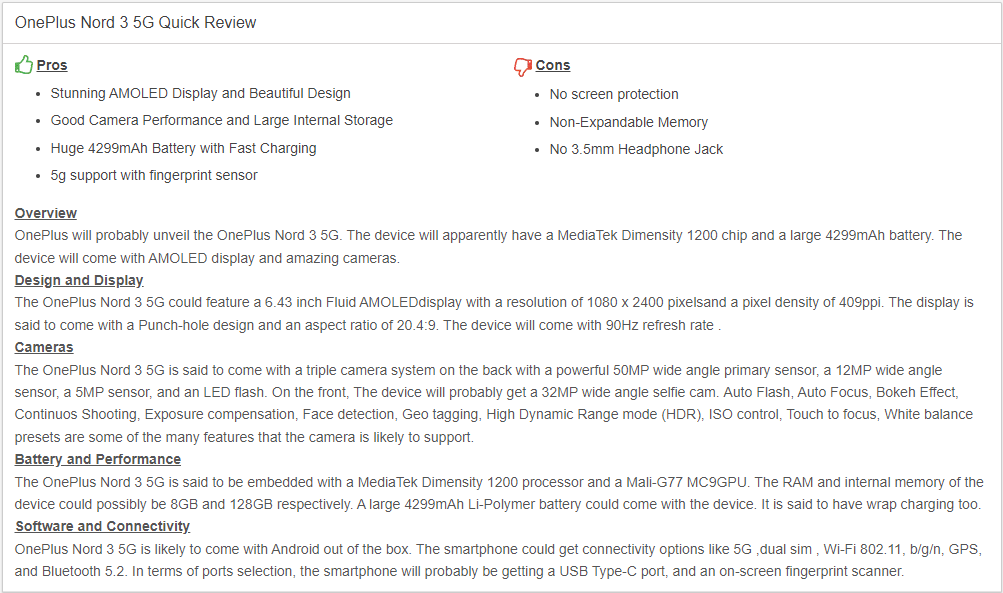
\includegraphics[width=12cm]{images/pricebaba_review_structure.png}
    \caption{pricebaba reviews structure \citep{OnePlusNord35G2023}}
    \label{fig:pricebaba-review-structure}
\end{figure}
\begin{figure}[H]
    \centering
    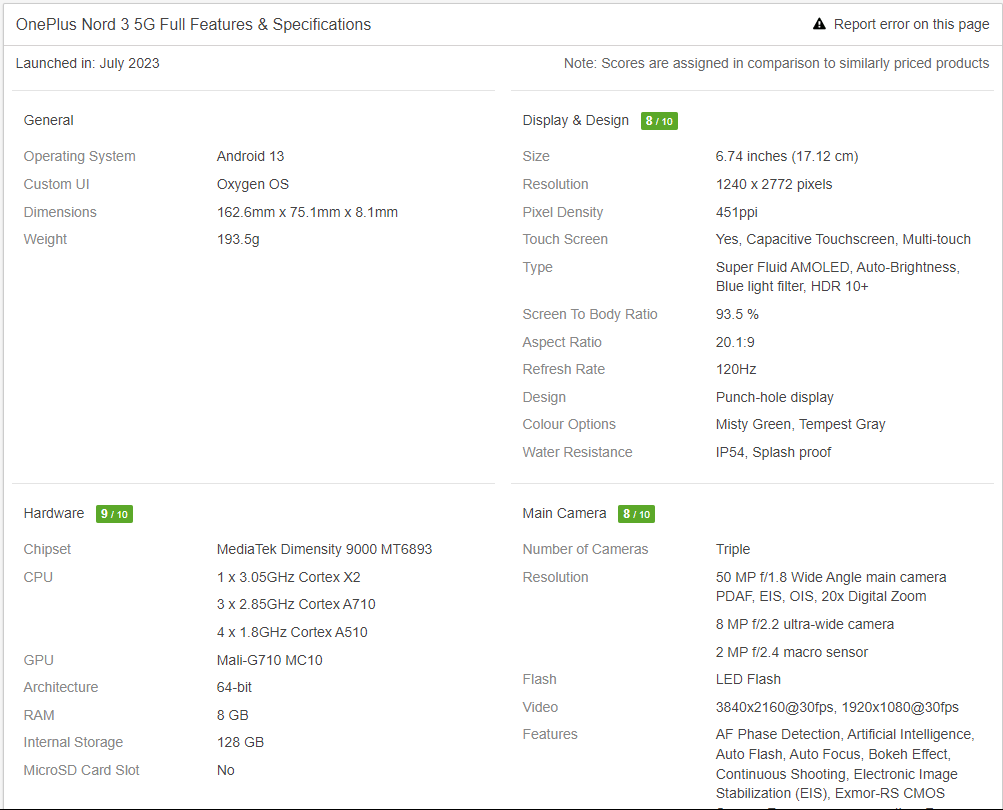
\includegraphics[width=12cm]{images/pricebaba_spec_structure.png}
    \caption{pricebaba specifications structure \citep{OnePlusNord35G2023}}
    \label{fig:pricebaba-spec-structure}
\end{figure}

\newpage
\begin{lstlisting}[style=jsonstyle, frame = single, caption=JSON Data Format Product specification, label=code:json-data-format]
{
    "url": {
        "keys_specifications": [],
        "full_specifications": [
            "Launch Date": "Launch Date",
            "General": {
                "subcategories1": [
                    "value1"
                    ],
                "subcategories2": [
                    "value1",
                    "value2"
                    ],
                ...
            },
            "Characteristic1": {
                "subcategories1": [
                    "value1"
                    ],
                "subcategories2": [
                    "value1",
                    "value2"
                    ],
                ...
            },
            "Characteristic2": {
                "subcategories1": [
                    "value1"
                    ],
                "subcategories2": [
                    "value1",
                    "value2"
                    ],
                ...
            },
            ...
        ]
    },
}
\end{lstlisting}
\newpage
\begin{lstlisting}[style=jsonstyle, frame = single, caption=JSON Data Format reviews, label=code:json-review-format]
{
    "url": {
        "text": {
            "Characteristic1": ["Description1"],
            "Characteristic2": ["Description2"],
            ...
        },
        "Pros": [
            "Pro 1",
            "Pro 2",
            "Pro 3"
        ],
        "Cons": [
            "Con 1",
            "Con 2",
            "Con 3"
        ]
    },
}
\end{lstlisting}

\subsection{Data Cleaning and Normalization}
To ensure consistency and usability, the extracted data underwent rigorous cleaning and normalization:
\begin{itemize}
    \item Standardizing all values to lowercase.
    \item Replacing special characters (e.g., `\&` with `and`).
    \item Reordering keys for logical and contextual coherence.
\end{itemize}
For instance, the key `Display \& Design` was transformed into `Design and Display` to improve readability.

\subsection{Data Integration}
The reviews and specifications JSON files were merged into a unified dataset by matching entries based on their unique product URLs. This ensured that each product's reviews and specifications were consolidated into a single cohesive data entry.

\subsection{Data Filtering}
Irrelevant and redundant entries were removed to refine the dataset further:
\begin{itemize}
    \item Discarding reviews with no textual content in the `text` field.
    \item Removing specifications containing only generic data, such as entries labeled `General`.
    \item Excluding overly simplistic reviews categorized as `Overview`.
\end{itemize}

\subsection{Data Splitting}
The finalized dataset was divided into training and testing sets with an 80\%-20\% split. This ensured a sufficient volume of data for training while retaining a reliable subset for evaluation.

\section{Prompt Structuration}
\subsection{Prompts for Dataset 1 (eC-Tab2Text)}
Prompts were carefully designed to guide models in generating detailed, contextually relevant reviews based on specific product attributes. Each prompt instructed the model to utilize key product features from the JSON-structured data and generate reviews adhering to the given keys. For example, a prompt could ask the model to focus on ``Design and Display'' and ``Battery.'' The dataset was expanded to approximately 12k high-quality prompts through key permutation strategies, facilitating extensive training and evaluation.

For this purpose, instructions with the following structure will be created:
\begin{lstlisting}[style=textstyle, frame = single, caption=Prompt structuration, label=code:prompt-structuration]
"Given following json that contains specifications of a product, generate a review of the key characteristics with json format. Follow the structure on Keys to write the Output: 
### Product: Product for JSON specifications
### Keys: Combination of the keys of the JSON reviews
### Output: reviews for JSON reviews accordingly to the keys"
\end{lstlisting}
it means that instructions will be generated for each permutation of the review keys. For example, if there is a review with the keys Design and Display', Camera', Battery', Performance', Software', i' instructions are chosen from the possible combinations of these keys, where i' is the number of instructions desired to be generated. This approach ensures that the model generates reviews according to the different characteristics of the products. An example of key selection could be that if a product has the keys Design and Display', Camera', Battery', Performance', Software', then the keys Design and Display', Camera' might be selected to generate one instruction, and for another instruction for the same product, the keys Design and Display', Battery' might be selected, and so on.
\\\\
With these combinations of keys for generating instructions, from the original 7,400 data points, 60,700 instructions are obtained that will be used to train the models. These instructions are the final dataset, which is available on \href{https://huggingface.co/datasets/kokujin/json_data_luis}{Hugginface}.

\begin{table}[ht]
    \footnotesize
    \centering
    \begin{tblr}{hline{1,2,Z} = 0.8pt, hline{3-Y} = 0.2pt,
                 colspec = {Q[l,m, 13em] Q[l,m, 6em]},
                 colsep  = 4pt,
                 row{1}  = {0.4cm, font=\bfseries, bg=gray!30},
                 row{2-Z} = {0.1cm},
                 }
    \textbf{Topic}       & \textbf{Value} \\ 
    \SetCell[c=2]{c} \textit{Input}\\
    \# Samples & 11,994\\
    Avg \# Attributes & 59.8\\
    Max \# Attributes & 68\\
    \SetCell[c=2]{c} \textit{Output}\\
    \# Queries & 3354\\
    Avg \# words/query & 56.61\\
    \end{tblr}
\caption{Statistics of eC-Tab2Text dataset}
\label{table:eC-Tab2Text-statistics}
\end{table}

\subsection{Prompts for Dataset 2 (QTSUMM)}
This dataset will be use to applied a cross-validation technique to evaluate the models. The data will be obtained for an existing dataset that is not product-based, but it is focused on structured data in JSON format. The dataset is QTSUMM \citep{zhao2023qtsummqueryfocusedsummarizationtabular}, which contains the columns: table, which contains JSON format data; query, which is the `keys' the model will use to generate the output; and summary, the expected output. The dataset is structured as shown in Figure \ref{fig:qsumm-structure}, where each object contains the columns especified before. This dataset will be used to generate prompts for the models to evaluate their performance.

\begin{figure}[H]
    \centering
    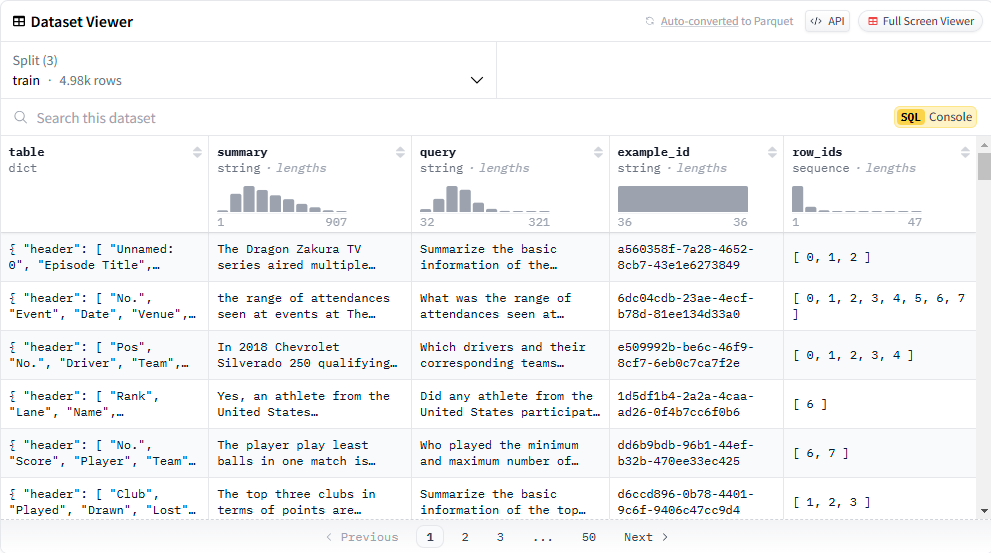
\includegraphics[width=12cm]{images/qsumm_structure.png} 
    \caption{QTSUMM dataset structure \citep{zhao2023qtsummqueryfocusedsummarizationtabular}}
    \label{fig:qsumm-structure}
\end{figure}

For QTSUMM, prompts were structured similarly but adapted to its unique characteristics. The `prompts` column in QTSUMM was filled with data derived from the `table`, `query`, and `summary` columns, ensuring the model understood instructions regardless of the dataset used.

For the QTSUMM dataset, the `prompts' column will be filled with data as follows:
\newpage
\begin{lstlisting}[style=textstyle, frame = single, caption=Prompt structuration, label=code:prompt-structuration]
"Given following json that contains specifications of a product, generate a review of the key characteristics with json format. Follow the structure on Keys to write the Output: 
### Product: Column table of JSON specifications
### Keys: Column query of the dataset
### Output: Column summary of the dataset"
\end{lstlisting}
The `prompt' as shown have the same format for both dataset, but the data used to fill them are different. This will allows the models understands the instructions no matter the dataset used to train or evaluate them.

\section{Model Fine-Tuning}

The eC-Tab2Text dataset provides a diverse and robust set of inputs and outputs, as summarized in Table~\ref{table:eC-Tab2Text-statistics}. The input JSON files contain rich attribute-based product specifications, with an average of 59.8 attributes per product and a maximum of 68 attributes for the most detailed entries. On the output side, the queries are designed to be concise and precise, with an average word count of 22.5 per query, enabling focused evaluation and training of the LLMs.

\subsection{eC-Tab2Text Evaluation} 
\label{sec:evaluation}

\paragraph{Model Selection and Characteristics} To evaluate the effectiveness of the eC-Tab2Text dataset, we fine-tuned three open-source LLMs: \textbf{LLaMA 2-Chat 7B} \cite{touvron2023llama}, \textbf{Mistral 7B-Instruct} \cite{jiang2023mistral}, and \textbf{StructLM 7B} \cite{zhuang2024structlm}. These models were selected due to their distinct pretraining paradigms, which address diverse data modalities and tasks. Detailed descriptions of these models are provided in Appendix \ref{sec:fine-tuning-models}.

\begin{itemize}
    \item \textbf{LLaMA 2-Chat 7B}: This model, pretrained on 2 trillion tokens of publicly available text data, is fine-tuned on over one million human-annotated examples. It excels in general-purpose conversational and language understanding tasks \cite{touvron2023llama}.
    \item \textbf{Mistral 7B-Instruct}: Leveraging a mix of text and code during training, this model demonstrates strong performance in tasks that require natural language understanding and programming-related reasoning \cite{jiang2023mistral}.
    \item \textbf{StructLM 7B}: Pretrained on structured data, including databases, tables, and knowledge graphs, StructLM is optimized for structured knowledge grounding, making it particularly effective for domain-specific tasks \cite{zhuang2024structlm}.
\end{itemize}

The fine-tuning process adapts these models to the e-commerce domain using the eC-Tab2Text dataset. This dataset focuses on attribute-specific and context-aware text generation tailored to user queries, such as detailed reviews of ``Camera'' or ``Design \& Display.'' The fine-tuning process follows best practices in instruction tuning and domain-specific dataset alignment \cite{Zhang2023InstructionTF, Chang2023ASO}. Optimization of hyperparameters ensured computational efficiency while maintaining high-quality performance, as detailed in Appendix Table~\ref{table:hyperparameters}.

\begin{table}[ht]
    \centering
    \footnotesize
    \begin{tabular}{|c|c|}
    \hline
    \textbf{Hyperparameter} & \textbf{Value} \\
    \hline
    Learning Rate & $2 \times 10^{-4}$ \\
    Batch Size & 2 \\
    Epochs & 1 \\
    Gradient Accumulation Steps & 1 \\
    Weight Decay & 0.001 \\
    Max Sequence Length & 900 \\
    \hline
    \end{tabular}
    \caption{Hyperparameter settings for fine-tuning.}
    \label{table:hyperparameters}
\end{table}

Furthermore, the `BitsAndBytesConfig` library from Hugging Face's `transformers` has been utilized for model optimization. These additional hyperparameters are shown in Table \ref{table:hyperparameters-bitsandbytes}.
\begin{table}[H]
    \centering
    \begin{tabular}{|c|c|}
        \hline
        \textbf{Hyperparameter} & \textbf{Value} \\
        \hline
        bnb\_4bit\_compute\_dtype & float16 \\
        bnb\_4bit\_quant\_type & nf4 \\
        use\_nested\_quant & False \\
        \hline
    \end{tabular}
    \caption{Hyperparameters Selection BitsAndBytes}
    \label{table:hyperparameters-bitsandbytes}
\end{table}

\paragraph{Metrics.} Evaluation metrics are essential for assessing the quality of text generation models. The most widely used metrics include: 

\begin{itemize} 
    \item \textbf{BLEU (Bilingual Evaluation Understudy)} \citep{Papineni02bleu:a}: Commonly used in machine translation and natural language generation, BLEU measures the overlap of n-grams between generated and reference texts. Despite its popularity, BLEU has limitations, particularly in capturing semantic similarity and evaluating beyond exact matches \citep{Reiter2018A}. 
    \item \textbf{ROUGE (Recall-Oriented Understudy for Gisting Evaluation)} \citep{lin-2004-rouge}: Focuses on recall-oriented evaluation by comparing the overlap of n-grams, word sequences, and word pairs between generated summaries and reference texts. It is highly effective for summarization tasks \citep{Ganesan2015ROUGE}.
    \item \textbf{METEOR (Metric for Evaluation of Translation with Explicit ORdering)}\citep{10.5555/1626355.1626389}: Incorporates stemming, synonymy, and flexible matching, providing a more nuanced evaluation than BLEU. It strongly correlates with human judgments, especially in translation tasks \citep{Dobre2015ACB}. 
    \item \textbf{BERTScore} \citep{zhang2020bertscoreevaluatingtextgeneration}: Leverages contextual embeddings from pre-trained transformer models to measure semantic similarity between generated and reference texts. Unlike n-gram-based metrics, BERTScore captures meaning and context, offering a robust evaluation for text generation tasks \citep{zhang2020bertscoreevaluatingtextgeneration}.
\end{itemize}

\paragraph{Prometheus Evaluation (Hallucination)} 
\label{appendix:Prometheus}
To evaluate model-based metrics, the Prometheus framework \citep{kim2024prometheus2opensource} was employed and an open-source LLM-based evaluator as an alternative to the closed-source G-Eval \cite{liu2023gevalnlgevaluationusing}. This evaluation was made utilizing structured prompts for three key evaluation criteria: fluency, correctness, and faithfulness \footnote{https://github.com/prometheus-eval/prometheus-eval}. The primary framework leverages an Absolute System Prompt, which defines the role of the evaluator and ensures objective, consistent assessments based on established rubrics. This Absolute System Prompt, shown in Listing\ref{code:ABS-System-Prompt}, forms the foundation for all evaluations across metrics. Our objective is to benchmark the performance of various LLMs under both zero-shot and fine-tuned settings using the proposed eC-Tab2Text dataset. 

\begin{lstlisting}[style=textstyle, frame = single, caption=Absolute System Prompt \citep{kim2024prometheus2opensource}, label=code:ABS-System-Prompt]
You are a fair judge assistant tasked with providing clear, objective feedback based on specific criteria, ensuring each assessment reflects the absolute standards set for performance.
\end{lstlisting}
The task descriptions for evaluating fluency, correctness, and faithfulness share a similar structure, as shown in Listing\ref{code:Task-description-Faithfulness},\ref{code:Task-description-fluency-correctness}. These instructions define the evaluation process, requiring detailed feedback and a score between 1 and 5, strictly adhering to a given rubric.

\vspace{15pt}

\begin{lstlisting}[style=textstyle, frame = single, caption=Task description used for evaluation of faithfulness \citep{kim2024prometheus2opensource}, label=code:Task-description-Faithfulness]
###Task Description:
An instruction (might include an Input inside it), a response to evaluate, a reference answer that gets a score of 5, and a score rubric representing a evaluation criteria are given.
1. Write a detailed feedback that assess the quality of the response strictly based on the given score rubric, not evaluating in general.
2. After writing a feedback, write a score that is an integer between 1 and 5. You should refer to the score rubric.
3. The output format should look as follows: "Feedback: (write a feedback for criteria) [RESULT] (an integer number between 1 and 5)"
4. Please do not generate any other opening, closing, and explanations.
5. Only evaluate on common things between generated answer and reference answer. Don't evaluate on things which are present in reference answer but not in generated answer.
\end{lstlisting}

\begin{lstlisting}[style=textstyle, frame = single, caption=Task description used for evaluation of fluency and correctness \citep{kim2024prometheus2opensource}, label=code:Task-description-fluency-correctness]
###Task Description:
An instruction (might include an Input inside it), a response to evaluate, a reference answer that gets a score of 5, and a score rubric representing a evaluation criteria are given.
1. Write a detailed feedback that assess the quality of the response strictly based on the given score rubric, not evaluating in general.
2. After writing a feedback, write a score that is an integer between 1 and 5. You should refer to the score rubric.
3. The output format should look as follows: "Feedback: (write a feedback for criteria) [RESULT] (an integer number between 1 and 5)"
4. Please do not generate any other opening, closing, and explanations.
\end{lstlisting}

\paragraph{Faithfulness prompt for model-based evaluation}

\begin{lstlisting}[style=textstyle, frame = single, caption=Prompt structured correctness \citep{kim2024prometheus2opensource}, label=code:estructured-faithfulness]
###The instruction to evaluate:
Evaluate the fluency of the generated JSON answer.
###Context:
{Prompt}
###Existing answer (Score 5):
{reference_answer}
###Generate answer to evaluate:
{response}
###Score Rubrics:
"score1_description":"If the generated answer is not matching with any of the reference answers and also not having information from the context.",
"score2_description":"If the generated answer is having information from the context but not from existing answer and also have some irrelevant information.",
"score3_description":"If the generated answer is having relevant information from the context and some information from existing answer but have additional information that do not exist in context and also do not in existing answer.",
"score4_description":"If the generated answer is having relevant information from the context and some information from existing answer.",
"score5_description":"If the generated answer is matching with the existing answer and also having information from the context."}
###Feedback:
\end{lstlisting}

\paragraph{Fluency prompt for model-based evaluation}

\begin{lstlisting}[style=textstyle, frame = single, caption=Prompt structured fluency \citep{kim2024prometheus2opensource}, label=code:estructured-fluency]
###The instruction to evaluate: Evaluate 
the fluency of the generated JSON answer
###Response to evaluate: {response}
###Reference Answer (Score 5): 
{reference_answer}
###Score Rubrics:
"score1_description":"The generated JSON answer is not fluent and is difficult to understand.",
"score2_description":"The generated JSON answer has several grammatical errors and awkward phrasing.",
"score3_description":"The generated JSON answer is mostly fluent but contains some grammatical errors or awkward phrasing.",
"score4_description":"The generated JSON answer is fluent with minor grammatical errors or awkward phrasing.",
"score5_description":"The generated JSON answer is perfectly fluent with no grammatical errors or awkward phrase
###Feedback:
\end{lstlisting}

\paragraph{Correctness prompt for model-based evaluation}

\begin{lstlisting}[style=textstyle, frame = single, caption=Prompt estructured correctness \citep{kim2024prometheus2opensource}, label=code:estructured-correctness]
###The instruction to evaluate:
Your task is to evaluate the generated answer and reference answer for the query: {Prompt}
###Response to evaluate:
{response}
###Reference Answer (Score 5):
{reference_answer}
###Score Rubrics:
"criteria": "Is the model proficient in generate a coherence response",
"score1_description": "If the generated answer is not matching with any of the reference answers.",
"score2_description": "If the generated answer is according to reference answer but not relevant to user query.",
"score3_description": "If the generated answer is relevant to the user query and reference answer but contains mistakes.",
"score4_description": "If the generated answer is relevant to the user query and has the exact same metrics as the reference answer, but it is not as concise.",
"score5_description": "If the generated answer is relevant to the user query and fully correct according to the reference answer.

###Feedback: 
\end{lstlisting}

The goal to apply cross-validation is to evaluate the robustness and generalizability of the fine-tuned models by testing them across distinct datasets. To achieve this, the same architectures trained with \textbf{eC-Tab2Text} dataset were evaluated on the \textbf{QTSumm} dataset \citep{zhao2023qtsummqueryfocusedsummarizationtabular}(\textbf{Llama2-chat 7B}, \textbf{StructLM 7B}, and \textbf{Mistral\_Instruct 7B}), using identical hyperparameters as detailed in Section~\ref{sec:evaluation}.
\paragraph{\textit{QTSumm Dataset.}\label{par:Prompt QTSumm}\citep{zhao2023qtsummqueryfocusedsummarizationtabular}} This dataset was design for query-focused summarization tasks, it includes structured tabular data, queries, and summaries over 2934 tables. This dataset in comparison to eC-Tab2Text, is focus on general-purpose summarization rather than product-specific reviews. The prompts uses to train the models with QTSumm dataset, has the same structure as the ones used to \textbf{eC-Tab2Text}. The difference lies in the QTSumm setup was the row-level content included in the prompts, as outlined in \ref{code:Prompt Dataset 2}.

\begin{lstlisting}[style=textstyle, frame = single, caption=Prompt structuration for QTSumm, label=code:Prompt Dataset 2]
    "Given following json that contains specifications of a product, generate a review of the key characteristics with json format. Follow the structure on Keys to write the Output: 
    ### Product: Column table of JSON specifications
    ### Keys: Column query of the dataset
    ### Output: Column summary of the dataset"
    \end{lstlisting}

\section{Resume}
This section provides a detailed overview of the methodology used for generating product reviews on e-commerce platforms using Large Language Models (LLMs). It describes the entire process from data collection and preparation, where data was generated from scratch, meticulously cleaned, and structured for further processing.
\\

The section continues by detailing the model tuning techniques, including the selection of hyperparameters and optimization methods, tailored to match the computational limits of the hardware. This phase was essential for adapting the models to produce relevant product reviews. The effectiveness of these fine-tuned models was then measured using evaluation metrics such as BLEU, METEOR, and ROUGE to assess the quality of generated reviews against actual product reviews.